\documentclass{article}

\usepackage{fancyhdr}
\usepackage{setspace}
\usepackage{titlesec}
\usepackage{tocloft}
\usepackage{lipsum}
\usepackage[fleqn]{amsmath}
\usepackage{amssymb}
\usepackage{hyperref}
\usepackage{url}
\usepackage{graphicx}
\usepackage{geometry}
\usepackage{enumitem}
\usepackage{parskip}
\usepackage{chemfig}
\usepackage{pdfpages}
\usepackage{tikz}
\usepackage{fancybox}
\usepackage{makecell}
\usepackage{pgfplots}
\usepackage{soul}
\usepackage{multirow}
\usepackage{ulem}
\usepackage{wrapfig}
\usepackage{subcaption}
\usepackage[T1]{fontenc}
\usepackage{esvect}
\usepackage{xcolor}
\usepackage{booktabs}
\usepackage{array}
\usepackage{colortbl}
\usepackage[utf8]{inputenc}
\usepackage{csquotes}
\usepackage{fontspec}
\usepackage[style=apa, backend=biber]{biblatex}
\usetikzlibrary{arrows}
\usetikzlibrary{decorations.pathreplacing}
\pgfplotsset{compat=1.17}
\definecolor{darkgreen}{RGB}{0, 160, 0}

\geometry{
    a4paper,
    total={170mm, 257mm},   
    left=20mm,
    top=20mm
}   

\hypersetup{
    colorlinks=true,
    linkcolor=black,
    urlcolor=blue,
    pdftitle={Team 31_Review 3 HS24}
}

\pagestyle{fancy}
\fancyhf{}
\fancyhead[L]{\leftmark}
\fancyhead[R]{\thepage}
\renewcommand{\headrulewidth}{0.4pt}
\newcommand{\figbox}[1]{ 
    \begin{figure*}[ht!]        
        \begin{center}            
            \fbox{#1}        
        \end{center}    
    \end{figure*}
}

\newcommand{\wrapfill}{
    \par
    \ifnum \value{WF@wrappedlines} > 0
        \addtocounter{WF@wrappedlines}{-1}%
        \null\vspace{
            \arabic{WF@wrappedlines}
            \baselineskip
        }
        \WFclear
    \fi
    \phantom{}
}

\newcommand{\difference}{\,\backslash\,}
\newcommand{\rem}{\underline{Remark}: }
\newcommand{\nots}{\underline{Notation}: }
\newcommand{\prf}{\underline{Proof}: }
\newcommand{\exs}{\underline{Example}: }
\newcommand{\defs}{\underline{Definition}: }
\newcommand{\wrn}{\underline{Warning}: }
\newcommand{\sht}{\ |\ }
\newcommand{\pph}[1]{\paragraph{#1} \phantom{}\\}
\newcommand{\dm}{\displaystyle}
\newcommand{\rad}{^{\mathrm{c}}}

\titleformat{\chapter}[block]{\bfseries\Large}{\thechapter.}{1em}{}

%========= TEXT ===========

\begin{document}

\hypersetup{citecolor=black}

\begin{titlepage}
    \begin{flushleft}
        \hspace*{.01cm}
        
\includegraphics[width=.3\textwidth]{media/hslu-logo-2.png}

        \vspace*{.01cm}
        \hspace*{.16cm}
\includegraphics[width=0.4\textwidth]{media/hslu-svg-logo.png}
    \end{flushleft}

    \vspace*{-.4cm}
    {\huge \textbf{Project Context 1}}

    {\Large Review 3}

    \vspace*{3cm}
    \begin{center}
        {\Huge \textbf{My$_{\text{celium}}$Tent}}

        \vspace*{.1cm}
        \textbf{\large The biodegradable tent}

%        \vspace*{.5cm}
%        \includegraphics*[width=.35\textwidth]{media/mytent_logo.png}
    \end{center}

    \vfill
    {\Large \textbf{Team 31}}\\
    {\large \vspace*{.01cm}
        Althaus Simon\\
        \vspace*{.01cm}
        Berner Nic\\
        \vspace*{.01cm}   
        Frongillo Matteo\\
        \vspace*{.01cm}
        McCarthy Benjamin\\
        \vspace*{.01cm}
        Nyamdorj Narandavaa\\
        \vspace*{.01cm}
    }
    
    \vspace{1cm}
    {\large Horw, 14th October 2024}
\end{titlepage}

\tableofcontents
\thispagestyle{empty}

\vspace*{1cm}
\section{Introduction}
The My$_{\text{celium}}$Tent addresses the need for sustainable alternatives in the
festival market, offering a biodegradable and affordable solution to reduce plastic waste
from abandoned tents. Made from mycelium-based materials, it minimizes the environmental
footprint while maintaining functionality for short-term camping. This project explores
the feasibility of biodegradable tents, evaluates design options, and aims to develop a
sustainable product that provides a comfortable camping experience. It includes
morphological analyses, a value-benefit assessment, and a rough description of the mock-up
to ensure the most effective design.

\newpage
\vspace*{-1.7cm}\section{File Note Review 2}
\begin{figure}[ht!]
    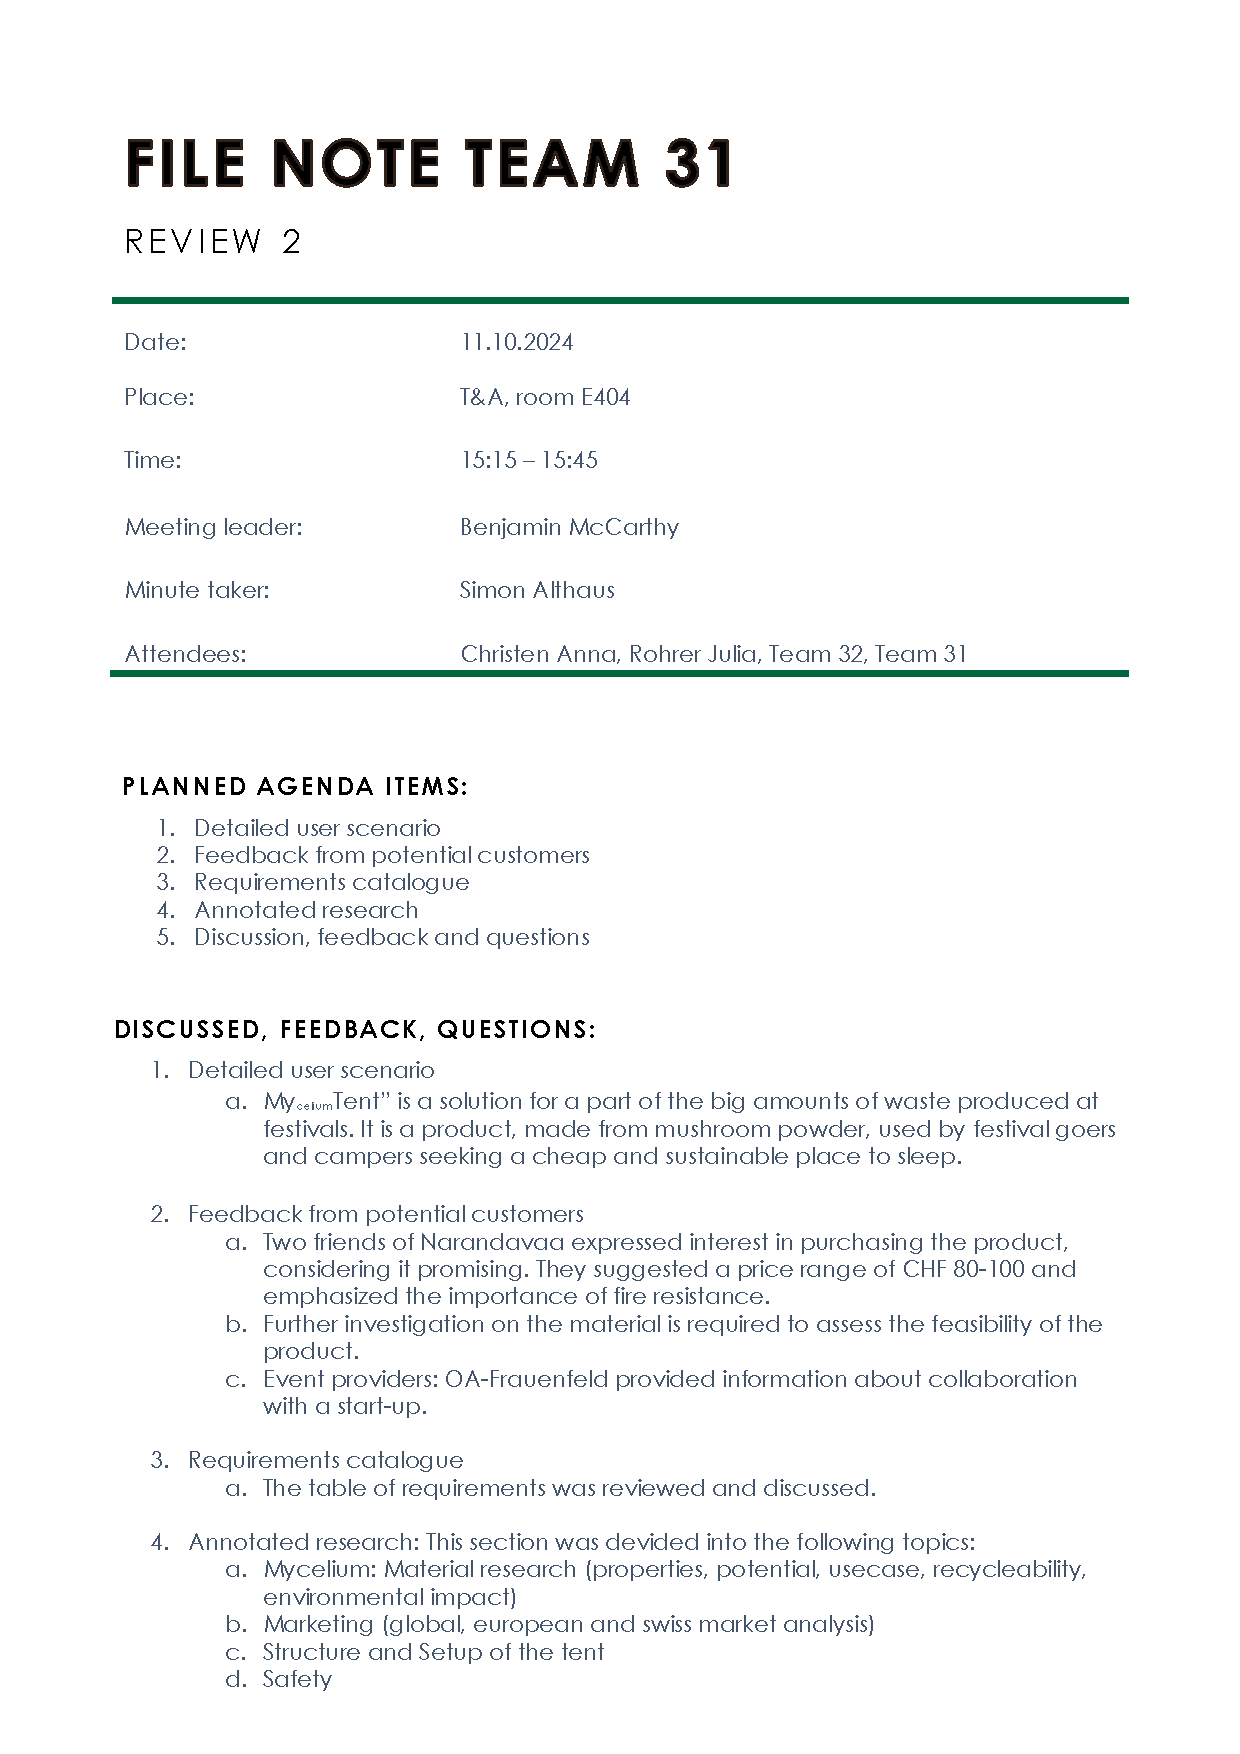
\includepdf[pages=1]{media/File Note Review 2.pdf}
\end{figure}
\newpage
\begin{figure}[ht!]
    \includepdf[pages=2]{media/File Note Review 2.pdf}
\end{figure}
\newpage

\section{Morphological Analysis}
The goal of this chapter is to produce three solution variants for a biodegradable festival
tent. Using the morphological box method, key design parameters were explored to
generate a range of possible solutions. From these, three promising variants were selected
for further evaluation based on their feasibility, sustainability, and alignment with the
project’s goals.

\subsection{Initial Morphological Box}
Table 1 presents the initial morphological box, which compiles the results of the
brainstorming session. Each row in the table represents a key design factor related to the
development of a biodegradable festival tent. For each factor, 3 to 4 possible solutions were
generated, reflecting a diverse range of materials, structural designs, and manufacturing
techniques. This systematic approach provided a comprehensive set of solution
combinations, which served as the foundation for selecting the most promising design
variants for further evaluation

\begin{table}[h]
    \caption{Initial Morphological Box}
    \centering
    \setlength{\arrayrulewidth}{1pt} % Set the line thickness
    \setlength{\tabcolsep}{5pt} % Adjust column padding
    \renewcommand{\arraystretch}{1.5} % Adjust row height
    \begin{tabular}{|>{\columncolor{gray!40}}p{3cm}|p{3cm}|p{3cm}|p{3cm}|p{3cm}|}
        \hline \rowcolor{cyan!30}
        \cellcolor{gray!20} \textbf{Sub-Functions / Problems} & \textbf{Solution 1} & \textbf{Solution 2} & \textbf{Solution 3} & \textbf{Solution 4} \\ \hline
        Shape & Right triangular prism & Dome & Tunnel & Instant-tent (Decathlon-Style) \\ \hline
        Size (People) & Max. 1 p. & Max. 2 p. & Max. 3 p. & Max. 4 p. \\ \hline
        Design & Single color & Multiple colors & & \\ \hline
        Structure support & Mycelium poles & Aluminum & Bamboo & Plastic \\ \hline
        Lifespan & Single use & 5 months & 1 - 3 years & \\ \hline
        Quality & Low & Medium & High & \\ \hline
        Processing Method & Mycelium-based Leather (MBL) & Unprocessed (MBC) & Kombucha leather & \\ \hline
        Duration of Biodegradation & 1 - 2 months & 3 - 12 months & 1 - 3 years & \\ \hline
    \end{tabular}
    \label{tab:morphological-box}
\end{table}

\newpage
\subsection{Elimination of subtopics}
This chapter focuses on the elimination of specific subfunctions, problems, and solutions to
streamline the design process. These eliminations were made to provide a clearer overview
of the most promising solution variants and to discard any illogical or impractical options. As
a result, Table 2 presents the slimmed-down version of the morphological box, highlighting
the refined set of feasible solutions for further consideration.

\begin{table}[h]
    \caption{Slimmed down Morphological Box}
    \centering
    \setlength{\arrayrulewidth}{1pt} % Set the line thickness
    \setlength{\tabcolsep}{5pt} % Adjust column padding
    \renewcommand{\arraystretch}{1.5} % Adjust row height
    \begin{tabular}{|>{\columncolor{gray!40}}p{3cm}|p{3cm}|p{3cm}|p{3cm}|p{3cm}|}
        \hline \rowcolor{cyan!30}
        \cellcolor{gray!20} \textbf{Sub-Functions / Problems} & \textbf{Solution 1} & \textbf{Solution 2} & \textbf{Solution 3} & \textbf{Solution 4} \\ \hline
        Shape & Right triangular prism & Dome & Tunnel & Instant-tent (Decathlon-Style) \\ \hline
        Size (People) & Max. 1 p. & Max. 2 p. & Max. 3 p. & Max. 4 p. \\ \hline
        {\vspace*{-.45cm}\color{red}{\st{Design}}} & {\vspace*{-.45cm}\color{red}{\st{Single color}}} & {\vspace*{-.45cm}\color{red}{\st{Multiple colors}}} & & \\ \hline
        Structure support & Mycelium poles & Aluminum & Bamboo & {\vspace*{-.45cm}\color{red}{\st{Plastic}}} \\ \hline
        Lifespan & Single use & 5 months & 1 - 3 years & \\ \hline
        Quality & Low & Medium & High & \\ \hline
        Processing Method & Mycelium-based Leather (MBL) & {\vspace*{-.45cm}\color{red}{\st{Unprocessed (MBC)}}} & Kombucha leather & \\ \hline
        {\vspace*{-.45cm}\color{red}{\st{Duration of Biodegradation}}} & {\vspace*{-.45cm}\color{red}{\st{1 - 2 months}}} & {\vspace*{-.45cm}\color{red}{\st{3 - 12 months}}} & {\vspace*{-.45cm}\color{red}{\st{1 - 3 years}}} & \\ \hline
    \end{tabular}
    \label{tab:slimmed-morphological-box}
\end{table}

The subfunction "Design" was removed, as the tent's color is not critical to the current
development phase and could be explored later as an additional feature. Similarly, the
duration of biodegradation was excluded, as this aspect will be evaluated separately in the
value-benefit analysis rather than during the solution-generation phase. Furthermore,
certain materials, such as unprocessed Mycelium-Based Composites (MBCs) and plastic,
were deemed illogical for this project. Unprocessed MBCs pose significant disadvantages
compared to processed materials like Mycelium-Based Leather (MBL), complicating the
tent's structural integrity. The use of plastic contradicts the project’s primary goal of
reducing plastic waste, making it unsuitable for consideration.

\subsubsection{Reduced Morphological Box}
Table 3 shows the reduced morphological box, after elimination of all the illogical solutions
and less important sub-functions or problems. After consideration of the remaining
solutions, three solution-variants were selected and inserted into the table.

\begin{table}[h]
    \caption{Reduced Morphological Box}
    \centering
    \setlength{\arrayrulewidth}{1pt} % Set the line thickness
    \setlength{\tabcolsep}{5pt} % Adjust column padding
    \renewcommand{\arraystretch}{1.5} % Adjust row height

    \begin{tikzpicture}[remember picture, overlay]
        \draw[blue, very thick, rounded corners]
        ([xshift=2mm, yshift=-2mm] -3.75, -1.5) --
        ([xshift=2mm, yshift=-2mm] 3.25, -3) --
        ([xshift=2mm, yshift=-2mm] -.3, -3.75) --
        ([xshift=2mm, yshift=-2mm] -.3, -4.25) --
        ([xshift=2mm, yshift=-2mm] -3.75, -5.3);

        \draw[darkgreen, very thick, rounded corners]
        ([xshift=2mm, yshift=-2mm] -.3, -1.5) --
        ([xshift=2mm, yshift=-2mm] 3.25, -2.25) --
        ([xshift=2mm, yshift=-2mm] -3.75, -3) --
        ([xshift=2mm, yshift=-2mm] -3.75, -5.15);

        \draw[orange, very thick, rounded corners]
        ([xshift=2mm, yshift=-2mm] 3.25, -1.5) --
        ([xshift=2mm, yshift=-2mm] 6.5, -2.25) --
        ([xshift=2mm, yshift=-2mm] -.3, -3) --
        ([xshift=2mm, yshift=-2mm] 3.25, -3.75) --
        ([xshift=2mm, yshift=-2mm] 3.25, -4.25) --
        ([xshift=2mm, yshift=-2mm] -3.75, -5.5);
    \end{tikzpicture}

    \begin{tabular}{|>{\columncolor{gray!40}}p{3cm}|p{3cm}|p{3cm}|p{3cm}|p{3cm}|}
        \hline \rowcolor{cyan!30}
        \cellcolor{gray!20} \textbf{Sub-Functions / Problems} & \textbf{Solution 1} & \textbf{Solution 2} & \textbf{Solution 3} & \textbf{Solution 4} \\ \hline
        Shape & Right triangular prism & Dome & Tunnel & Instant-tent (Decathlon-Style) \\ \hline
        Size (People) & Max. 1 p. & Max. 2 p. & Max. 3 p. & Max. 4 p. \\ \hline
        Structure support & Mycelium poles & Aluminum & Bamboo & \\ \hline
        Lifespan & Single use & 5 months & 1 - 3 years & \\ \hline
        Quality & Low & Medium & High & \\ \hline
        Processing Method & Mycelium-based Leather (MBL) & & Kombucha leather & \\ \hline
    \end{tabular}
    \label{tab:reduced-morphological-box}
\end{table}

\newpage
\subsection{Description of the three Solution Variants}
{\color{darkgreen}{Variant 1: Dome Tent (Single-Use, Fully Biodegradable)}}\\
The first variant is a dome-shaped tent, constructed entirely from biodegradable materials,
including mycelium poles and Mycelium-Based Leather (MBL). This variant is designed for
single-use and aims to provide the highest possible grade of biodegradability. It is produced
with a focus on low-cost and low-quality materials, suitable for short-term use at festivals.

{\color{orange}{Variant 2: Tunnel Tent (Four-Person, Long-Lasting)}}\\
The second variant is a tunnel tent, chosen for its optimal space-to-weight ratio, making it
suitable for accommodating four people—the largest capacity in this selection. It is designed
with higher-quality materials for a lifespan of one to three years, supported by an aluminum
structure for enhanced durability and stability.

{\color{blue}{Variant 3: Triangular Prism Tent (Two-Person, Medium-Lasting)}}\\
The third variant is a right triangular prism-shaped tent, designed for two people. This option
combines features from both the high-quality tunnel tent and the single-use dome tent. It
uses bamboo poles, which provide greater longevity than mycelium but are less durable
than aluminum, while still maintaining biodegradability.

The final selection between these three variants will be made in the following chapter.

\section{Value-Benefit Analysis}
Table 4 presents the Value-Benefit analysis of the three previously described tent variants. In
alignment with our primary objective of addressing plastic waste at festivals,
biodegradability is assigned the highest priority. The affordability of each variant is also
crucial, as it must remain competitive with existing products that contribute to the plastic
waste problem. Given that the target market is festival-goers seeking short-term, disposable
solutions, the overall quality and lifespan of the tents are less critical, as we do not aim to
compete in the high-quality tent market.

The analysis includes a row for "Weather Resistance," which evaluates the tent's ability to
endure adverse weather conditions, such as heavy winds. This aspect is particularly relevant
as different shapes provide varying levels of structural resilience.

\begin{table}[h]
    \caption{Value-Benefit Analysis}
    \centering
    \setlength{\arrayrulewidth}{1pt} % Set the line thickness
    \setlength{\tabcolsep}{5pt} % Adjust column padding
    \renewcommand{\arraystretch}{1.5} % Adjust row height

    \begin{tabular}{|p{3cm}|p{1.8cm}|>{\columncolor{green!20}}p{1cm}|>{\columncolor{green!20}}p{2cm}|>{\columncolor{orange!20}}p{1cm}|>{\columncolor{orange!20}}p{2cm}|>{\columncolor{cyan!20}}p{1cm}|>{\columncolor{cyan!20}}p{2cm}|}
        \hline
        \multirow{2}{*}{\cellcolor{cyan!30}} & \multirow{2}{*}{\cellcolor{cyan!30}} & \multicolumn{2}{c|}{\cellcolor{green!30}\textbf{Dome}} & \multicolumn{2}{c|}{\cellcolor{orange!30}\textbf{Tunnel}} & \multicolumn{2}{c|}{\cellcolor{cyan!30}\textbf{Prism}} \\ \cline{3-8}
        \textbf{Criteria}\cellcolor{cyan!30} & \textbf{Weighting}\cellcolor{cyan!30}& \textbf{Score} & \textbf{Weighted score} & \textbf{Score} & \textbf{Weighted score} & \textbf{Score} & \textbf{Weighted score} \\ \hline
        Price & 25 & 8 & 200 & 2 & 50 & 6 & 150 \\ \hline
        Biodegradability & 25 & 9 & 225 & 5 & 125 & 7 & 175 \\ \hline
        Handling & 15 & 6 & 90 & 5 & 75 & 6 & 90 \\ \hline
        Lifespan & 10 & 3 & 30 & 3 & 30 & 6 & 60 \\ \hline
        Quality & 10 & 3 & 30 & 8 & 80 & 6 & 60 \\ \hline
        Weather resistance & 15 & 7 & 105 & 7 & 105 & 5 & 75 \\ \hline
        \textbf{TOTAL Score} & & & \textbf{680} & & \textbf{515} & & \textbf{610} \\ \hline
    \end{tabular}
    \label{tab:value-benefit-analysis}
\end{table}

\subsection{Justified Choise}
Based on the weighted ratings derived from the Value-Benefit analysis (Table 4), the Dome
Tent variant emerges as the most suitable option, achieving a total score of 680 points,
which is by far the highest among the variants. Its strong alignment with our values of
biodegradability and affordability positions it effectively within the festival market. As such,
it represents the best solution to achieve our goal of mitigating plastic waste in festival
environments.

\newpage
\section{Rough Mock-up description}
The mock-up section presents a preliminary analysis of the purpose and essential details
of the tent. The goal is both to physically have a model of the tent and to serve as an
effective communication tool to convey the features and benefits of the tent to the target
audience, such as festival goers and outdoor enthusiasts.

\subsection{Purpose}
This mock-up of the My$_{\text{celium}}$Tent provides customers with an initial
impression of an attractive, affordable, biodegradable, and sustainable
solution to convetional tents.

\subsection{Target audience}
The target audience consist of individuals interested in festival and
outdoor events.

\subsection{Key Features / Sections}
The key features of the My$_{\text{celium}}$Tent include a dome-style structure
with space for two people, one main door, three small mesh windows for
airflow, and lightweight poles for structural support.

\subsection{Size}
\subsubsection{Tent size}
The My$_{\text{celium}}$Tent measures approximately 225 cm in length, 130 cm in width,
and 100 cm in height, providing sufficient space for two people.

\subsubsection{Mock-up size}
The mock-up is designed at a 1:10 scale to offer a clear understanding of the dimensions
and proportions of the final product.
\vspace*{-.2cm}
\begin{figure}[ht!]
    \centering
    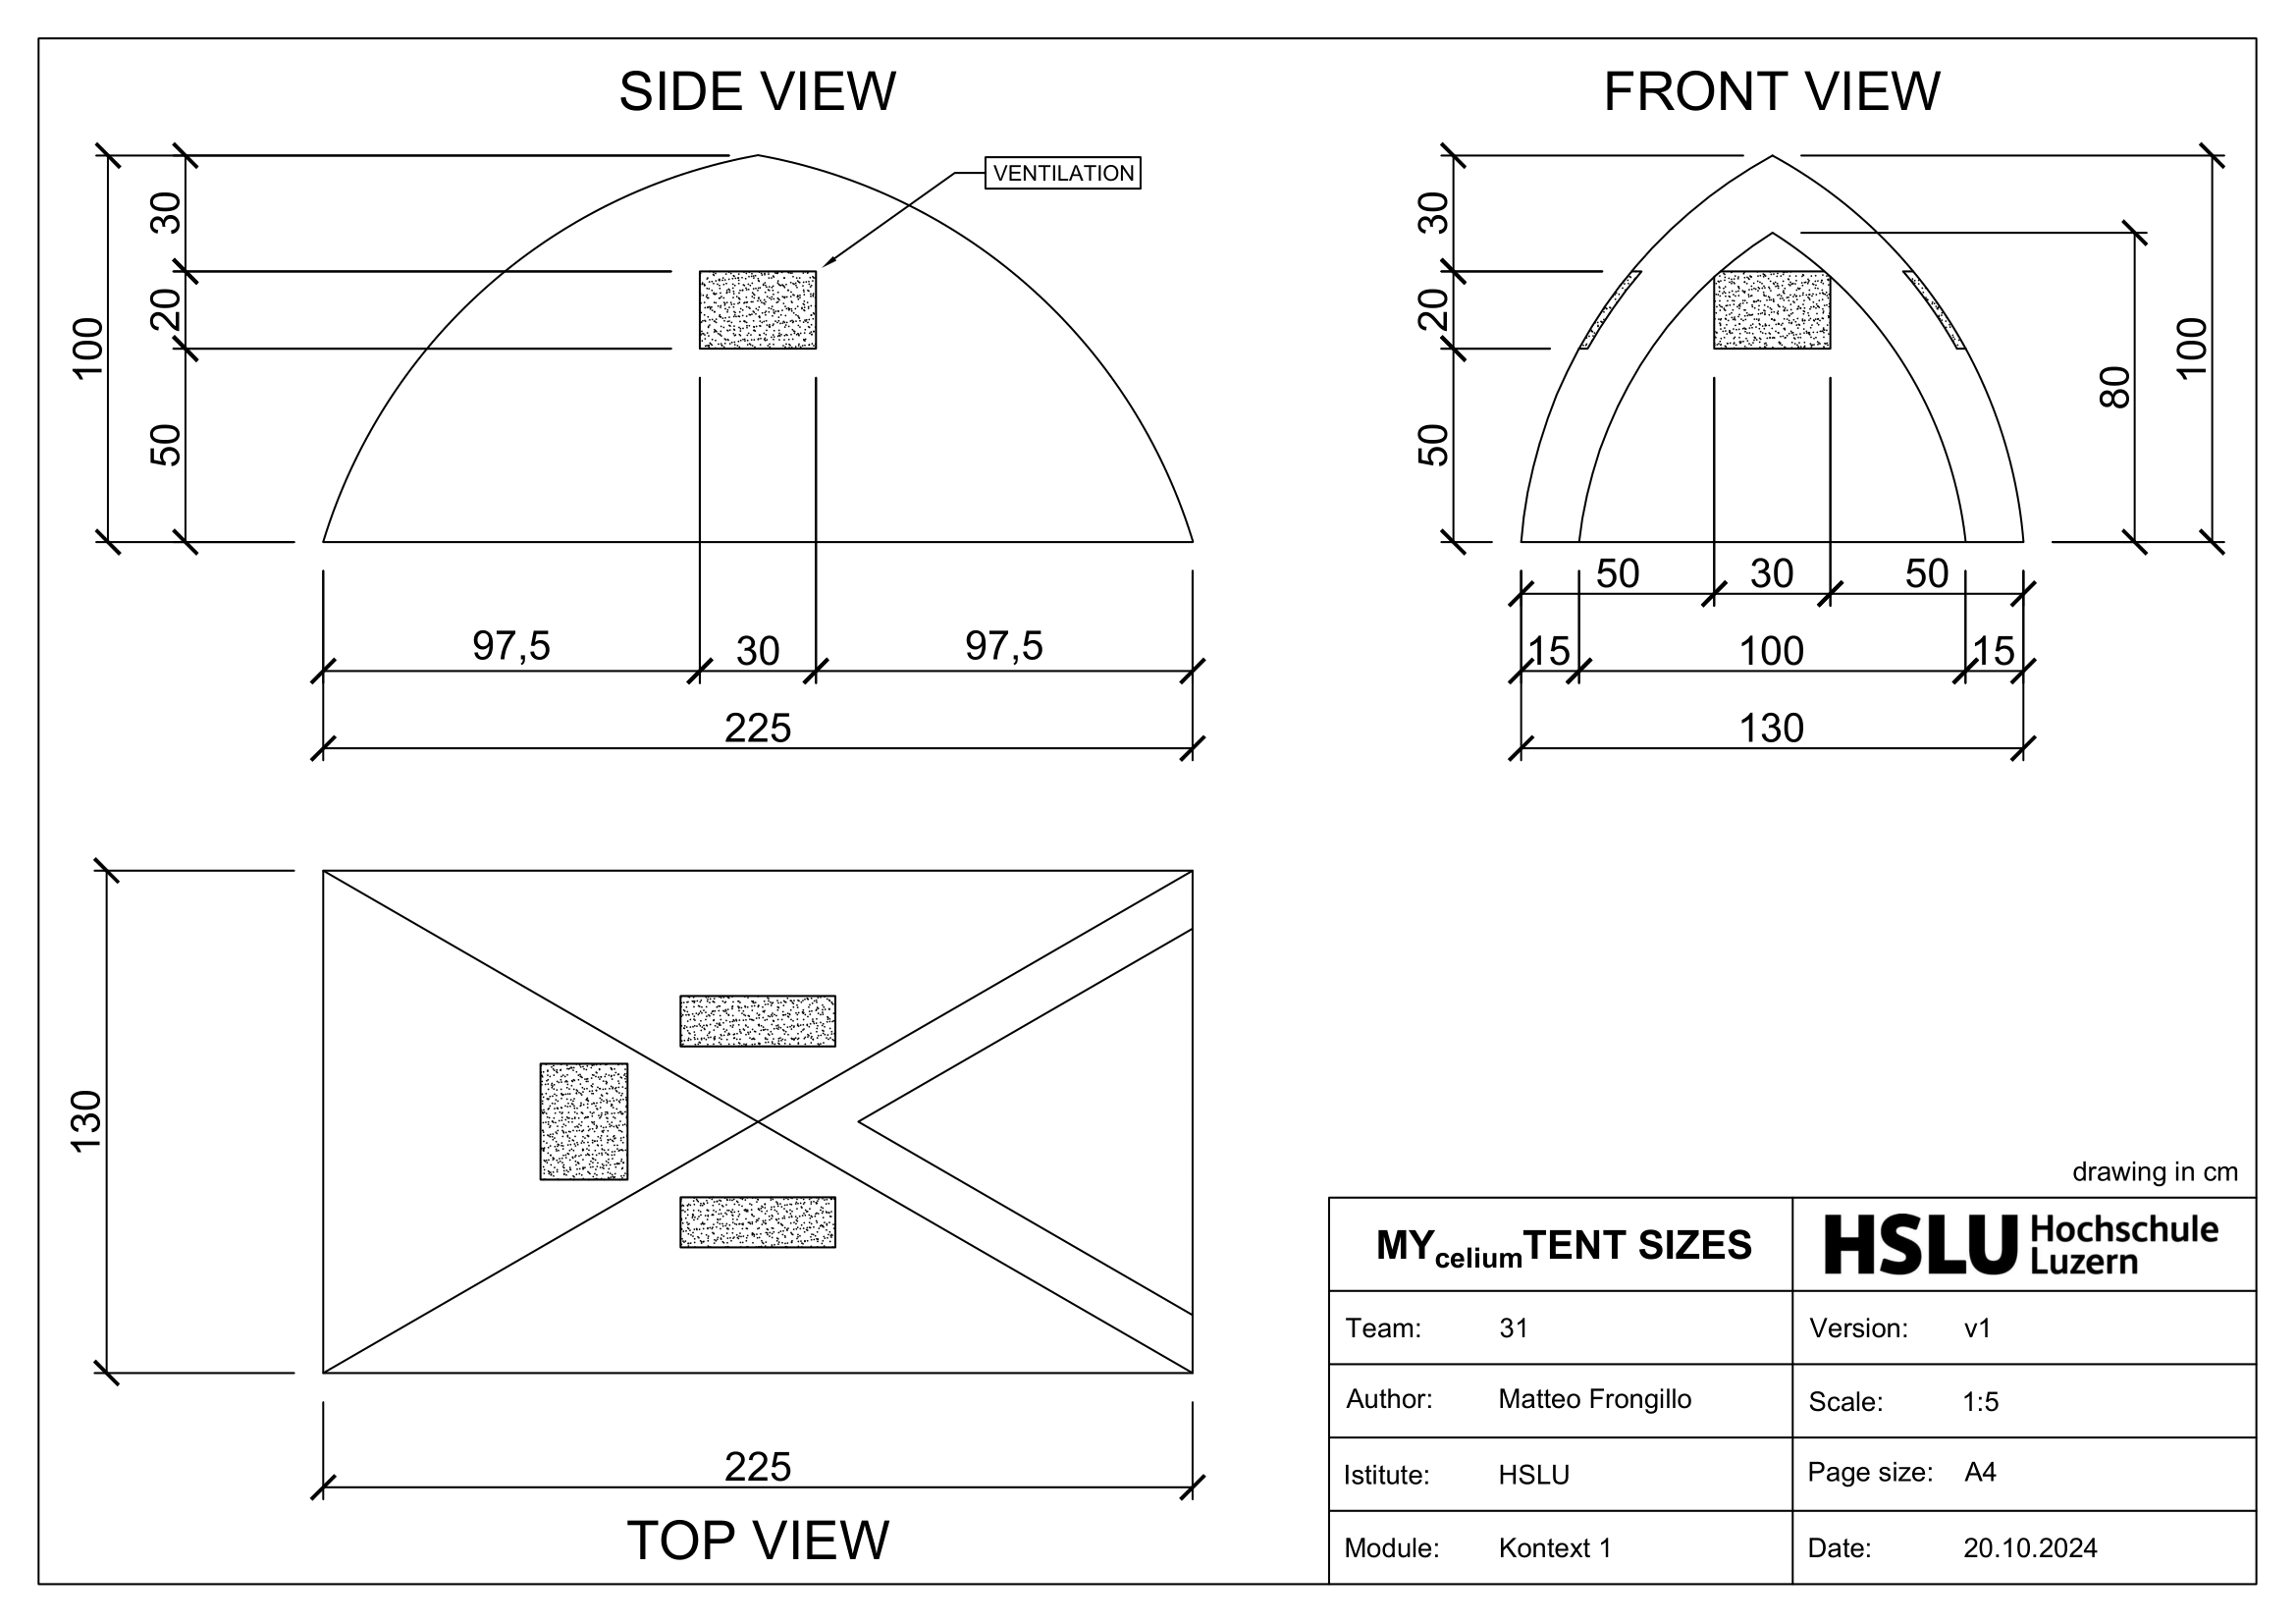
\includegraphics[width=\textwidth]{media/mytent-size.png}
    \caption{My$_{\text{celium}}$Tent dimensions and structure}
\end{figure}

\subsection{Rendering}
The 3D rendering of the MyCelium tent illustrates its dome configuration and context,
depicting the tent in a festival setting, showing its adaptability and integration in
these environments.

\begin{figure}[ht!]
    \centering
    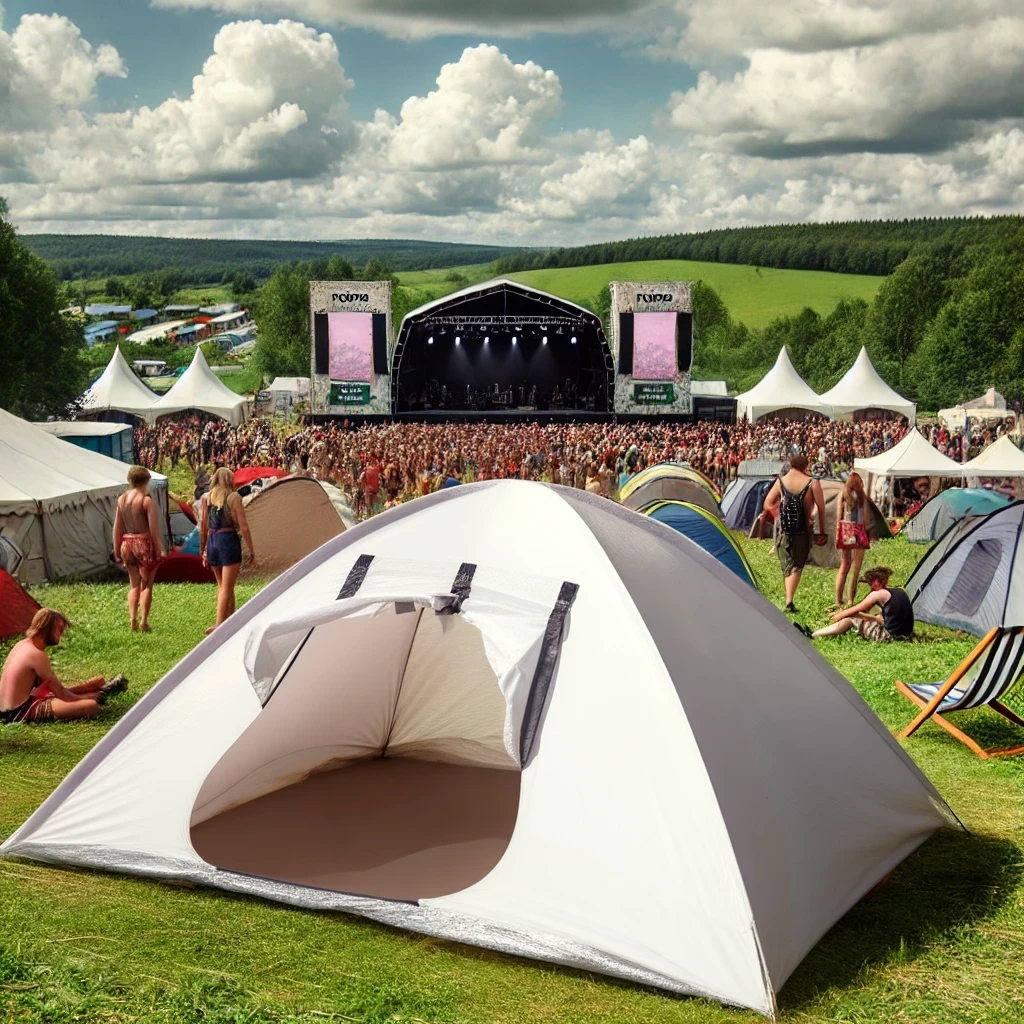
\includegraphics[width=.55\textwidth]{media/3d-tent-rendering.png}
    \caption{3D visualization of the Tent in the environment.}
\end{figure}

\section{Declarations on the use of AI tools}
\begin{itemize}
    \item \textit{DeepL} and \textit{ChatGPT 4o} have been used as a spell-checker;\\
        \url{https://www.deepl.com/}\\
        \url{https://www.chatgpt.com/}
\end{itemize}

\newpage
\listoftables

\listoffigures

\end{document}

